\section{Verifiable Credentials (VC)}

Verifiable Credentials (VCs) represent the third layer of the self-sovereign identity framework. 
\medskip

\noindent
VCs are digital credentials, conceptually similar to physical documents such as identity cards or driving licences, but expressed using a structured JSON-based data model. They are designed to support lifelong, secure, and rich identity descriptions, in line with the requirements defined for SSI systems.
\medskip

\noindent
The data model for verifiable credentials is defined by the W3C Verifiable Credentials Working Group and is currently specified in version-2.0. As with the DID specification, the model is extensible and supports custom vocabularies and domain-specific attributes.
\medskip

\noindent
A credential becomes “verifiable” because it is digitally signed by the issuer. This ensures authenticity, integrity, and resistance to tampering. Holders can generate a verifiable presentation by packaging one or more credentials and signing the presentation themselves. 
This presentation can then be shared with a verifier following either a two-party or three-party interaction model.

\subsection {Three- and Two-Party Interaction Models}

The most common interaction pattern for verifiable credentials is the 
\textbf{three-party model}, involving:
\begin{itemize}
    \item \textbf{Issuer}: creates and signs the verifiable credential.
    \item \textbf{Holder}: stores one or more credentials and generates 
    verifiable presentations by signing them.
    \item \textbf{Verifier}: receives the presentation and validates its 
    authenticity, integrity, and structure.
\end{itemize}

\noindent
The verifier performs several checks:
\begin{itemize}
    \item verifies the holder’s signature on the verifiable presentation,
    \item verifies the issuer’s signature on each embedded credential,
    \item validates the credential schema (typically published by the issuer on a VDR),
    \item relies on \textit{implicit trust} in the issuer, since no direct 
    interaction occurs between verifier and issuer during verification.
\end{itemize}

\noindent
This model reflects the SSI principle of peer-to-peer interactions: holders interact directly with issuers when obtaining credentials and with verifiers when proving their identity. \\
Verifiable credentials therefore contain the holder’s DID, which binds the credential to the subject and allows the verifier to retrieve the public key associated with the DID.
\medskip

\noindent
Although outside the scope of this module, verifiable credentials may also be combined with zero-knowledge proofs, enabling holders to prove certain properties without revealing all credential attributes.
\medskip

\noindent
A less common alternative is the \textbf{two-party model}, where issuer and verifier coincide. \\
The holder presents the credential back to the same entity that issued it. This model is used in niche scenarios, for example when credentials are employed to regulate access frequency or service usage.\\
However, the three-party model remains the standard for most SSI deployments.

\begin{figure}[h!]
    \centering
    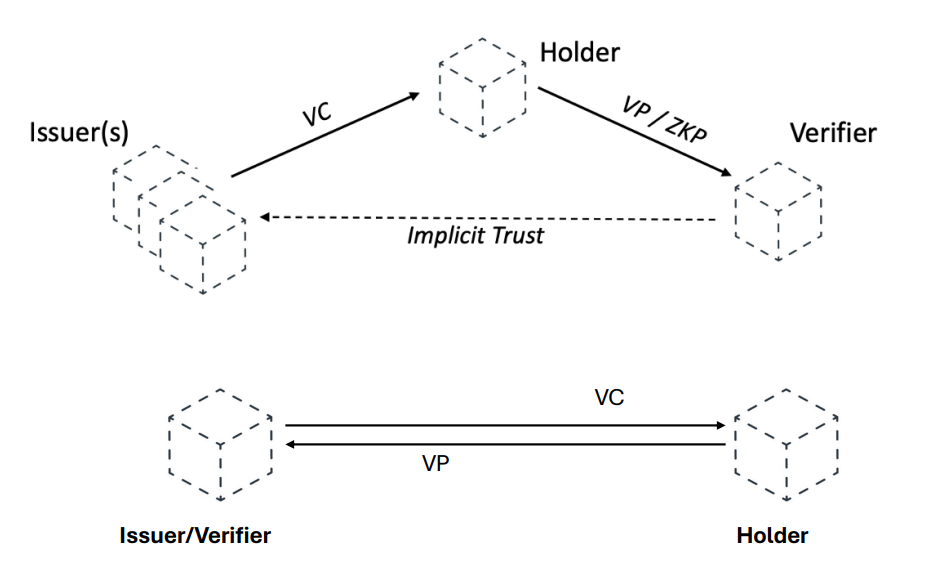
\includegraphics[width=0.85\textwidth]{images/section_5/three_two_party_models.png}
    \caption{Three-party model (top) and two-party model (bottom) for verifiable credential exchange.}
    \label{fig:vc-models}
\end{figure}


\subsection {Verifiable Data Registry (VDR)}

At the core of the verifiable credential ecosystem lies the 
\textbf{Verifiable Data Registry (VDR)}, which maintains the identifiers 
(e.g., DIDs) and the credential schemas required for interoperability.  
Even if a verifier trusts a specific issuer, it must still retrieve the 
schema of the credential in order to correctly interpret and validate the 
claims. For this reason, issuers typically publish credential schemas on 
the VDR.
\medskip

\noindent
In addition to identifiers and schemas, the VDR may also maintain 
\textbf{revocation information}, enabling verifiers to check whether a 
credential is still valid. Although not shown in all conceptual diagrams, 
revocation is an essential component of the full lifecycle of VCs.

\paragraph{Issuer.}
The issuer creates and signs verifiable credentials. Before issuing a 
credential, it verifies the holder’s identifier (e.g., the DID) by 
confirming control of the associated private key. Issuers also interact 
with the VDR to retrieve or publish credential schemas.

\paragraph{Holder.}
The holder acquires, stores, and presents verifiable credentials using a 
dedicated \textit{wallet}. The holder assembles verifiable presentations 
by wrapping credentials and signing the presentation with their own private 
key. The holder may also query the VDR to verify identifiers or schemas.

\paragraph{Verifier.}
The verifier validates incoming verifiable presentations by checking the 
holder’s signature, the issuer’s signature on each credential, schema 
 correctness, and—when applicable—revocation status.  
To perform these checks, the verifier queries the VDR for identifiers, 
schemas, and auxiliary validation data.

\medskip

\begin{figure}[h!]
    \centering
    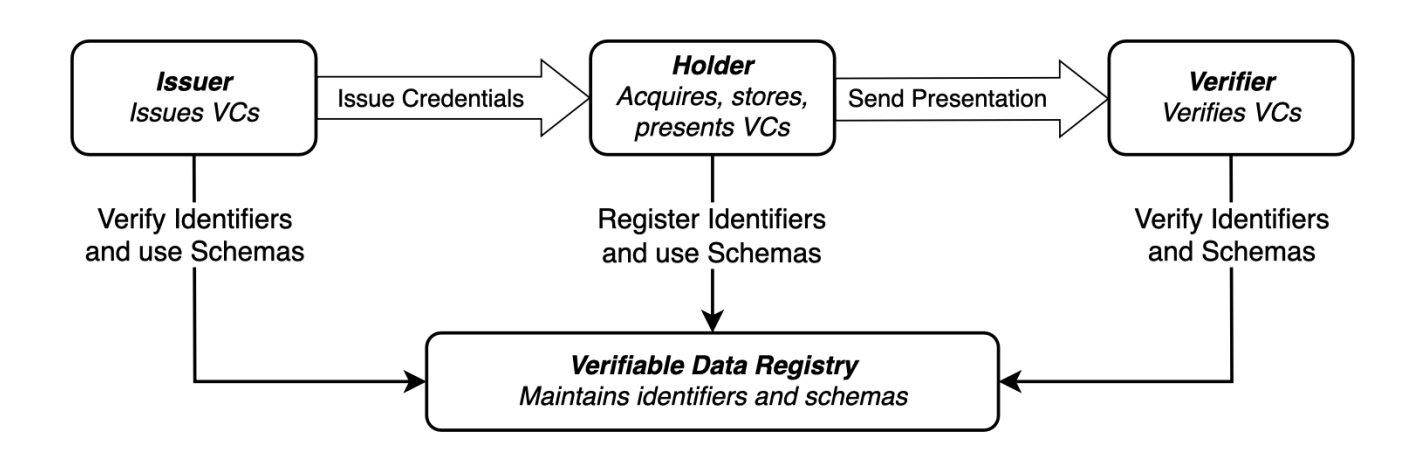
\includegraphics[width=0.92\textwidth]{images/section_5/roles_information_flow.png}
    \caption{Roles and information flow among issuer, holder, and verifier. 
    The Verifiable Data Registry maintains identifiers, schemas, and revocation data.}
    \label{fig:vc-roles-flow}
\end{figure}
